
By way of guiding the user on how to best exploit the CFS plugin, we will focus on two applications from the CESAR suite of exascale proxy applications \cite{CESAR}, NEKBONE and MOCFE. The NEKBONE proxy application is a thermal hydraulics simulation code for  reactor simulations that solves the Poisson equation, Helmholz equation, as well as other differential equations. It is an MPI-based FORTRAN application consisting of 13 files. For the example discussed here, the application was executed with 8 processes and 50 elements per process, a polynomial order of 10, and without the multi-grid preconditioner (i.e. `Example~3' in the provided source code). 

The MOCFE application simulates the main procedures in a 3D method of characteristics (MOC) code for numerical solution of the steady state neutron transport equation.  3D-MOC features heterogeneous geometry capability, high degree of accuracy, and potential for scalability. It is a FORTRAN~90 MPI application consisting of 36 files. We have instrumented the inner loop of {\tt Method\_FGMRES.F90} as a phase\_region of the application. For the example cases described here MOCFE was executed with 16 processes and a Krylov iteration size of 60.


\subsubsection{Using different search algorithms}\label{sec:cfs-search}

The CFS plugin searches for the best possible combination of compiler flags from a list of flags provided in the \texttt{cfs\_config.cfg} file of the plugin. It uses one of five search algorithms, i.e., \textit{Exhaustive Search}, \textit{Random Search}, \textit{Individual Search}, \textit{Genetic Search}, and \textit{Machine Learning-based Random Search} for selecting the best combination of flags. In general, the Individual Search strategy provides good results and is recommended as a good starting point. The Genetic Search and Random Search algorithms can be used in combination with Machine Learning to perform a broader search.

The search algorithms of the CFS plugin are described below:

\begin{itemize}
\item \textit{Exhaustive Search (ES):} The plugin compiles and executes the application with all combinations of the specified compiler flags.
\item \textit{Random Search (RS):} The plugin randomly selects combinations of flags.
\item \textit{Individual (IS):} This algorithm adds-up each compiler flag one after the other from the tuning parameter list in the order used  in the specification file.
\item \textit{Genetic Search (GS): } GS searches for the combination of compiler flags based on the GDE3 genetic algorithm.
\item \textit{Machine learning based Random Search (MLRS): } MLRS uses the Tuning Database of PTF, which is a collection of CFS tuning results for different applications, to model and predict the suitable compiler flags for the current application. The database, in our case, was filled with the NAS parallel benchmark experiments.
\end{itemize}

For the example cases discussed here, we can run all of these algorithms (apart from ES due to the huge number of scenarios) on the NEKBONE application. In the case of the NEKBONE application, the body of the progress loop in the NEKBONE application was marked as a User Region and we also use the following CFS plugin specific features: i) the \textit{Selective Make} option of the CFS plugin to recompile only compute intensive files instead of the entire application and ii) the \textit{Remote Make} option to perform the compilation on the login nodes of SuperMUC, the supercomputer at LRZ that we run our use cases on. For the use-cases described here the compiler flags were pre-defined in the {\tt cfs\_config.cfg} file of the CFS plugin.

We focus on the following FORTRAN compiler flags of Intel's {\tt ifort} compiler when auto-tuning NEKBONE using the CFS plugin:

\begin{verbatim}
tp "TP_IFORT_OPT" = "-" ["O2", "O3", "O4"];
tp "TP_IFORT_XHOST"  = " " ["-xhost", " "];
tp "TP_IFORT_UNROLL" = " " ["-unroll", " "];
tp "TP_IFORT_VERSION" = " " ["-opt-multi-version-aggressive", " "];
tp "TP_IFORT_FMA" = " " ["-fma", " "];
tp "TP_IFORT_INLINE" = " " ["-finline-functions","-fno-inline-functions"];
tp "TP_IFORT_PREFETCH" = "-opt-prefetch=" [1,4,1];
tp "TP_IFORT_UNROLL" = "-unroll" [1,16,4];
tp "TP_IFORT_OPTBLOCK" = "-opt-block-factor=" [1,3,1];
tp "TP_IFORT_STREAM" = " " ["-opt-streaming-stores always",
          "-opt-streaming-stores never", "-opt-streaming-stores auto"];
tp "TP_IFORT_IP" = " " ["-ip", " "];
\end{verbatim}

Figure~\ref{fig:nek_comparisons} compares the execution times for the different search algorithms for the NEKBONE application for a given number of experiments.

\begin{figure}
        \centering
        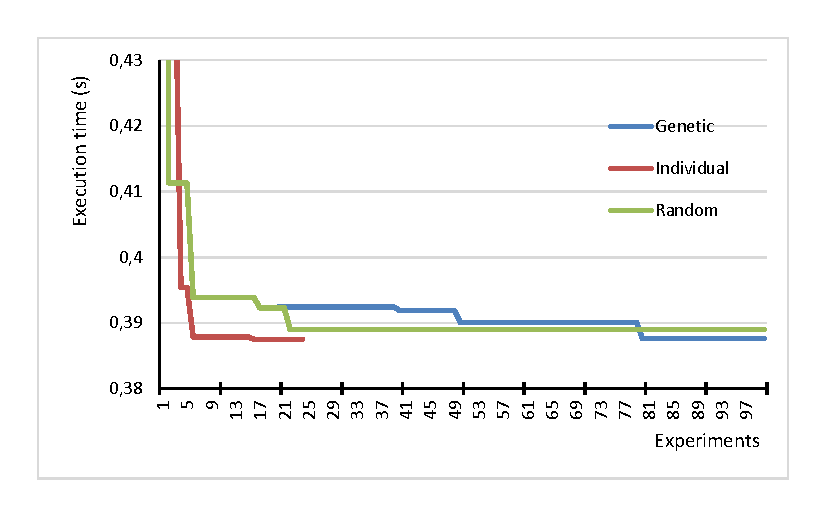
\includegraphics[width=13cm]{../BPG/CFS/CFS-Nekbone-Comparison.pdf}
         \caption{Comparison of IS, GS, and RS for NEKBONE.}
     \label{fig:nek_comparisons}
\end{figure}

It can be seen that all three search algorithms converge to approximately the same execution time for the instrumented application (~0.38 seconds). While the IS algorithm results in the best execution time after only five experiments, the RS algorithm requires 22 experiments and the GS algorithm requires 80 experiments to obtain the shortest execution time for the instrumented application, thus demonstrating the potential advantages of some search algorithms over others when using the CFS plugin. As mentioned, the Individual Search strategy generally provides good results and is recommended as a good starting point when employing the CFS plugin.

\subsubsection{Reducing the compilation time for selected flag combinations} \label{sec:cfs-selective-make}

The \textit {Selective Make} feature of the CFS plugin allows users to reduce the compilation time for a selected combination of flags by recompiling only significant target application files, i.e., files that account for most of the execution time. To demonstrate the impact of this feature here, we apply the CFS plugin (with Individual Search) to the NEKBONE and MOCFE applications . As can be seen from Table~\ref{tab:cfs-recompilation}, the compilation time for the applications differs significantly between recompiling the whole application and recompiling only the significant files using Selective Make. Indeed, for applications composed of many files the Selective Make feature generally leads to a significant reduction in the overhead of searching through CFS parameter spaces and is recommended to CFS plugin users to improve productivity.

\begin{table}
    \centering
    \begin{tabular}{|c | c| c | c | c |}
    \hline
      & \multicolumn{2}{c}{Full Compile} & \multicolumn{2}{|c|}{Selective Compile}\\\hline
     Code & \#Files & Time (s) & \#Files & Time (s)\\
    \hline\hline
    MOCFE	&36 &32.12& 4 &4.503\\[1ex]
    NEKBONE &13 &45.16 &1 &2.22\\[1ex]  \hline
    \end{tabular}
    \caption{Compilation time for the whole application relative to compilation time selecting only the most significant application files.}
\label{tab:cfs-recompilation}
\end{table}

Table~\ref{tab:cfs-selective-influence} compares the results running MOCFE and NEKBONE with the full compilation and the compilation using Selective Make. The results demonstrate that selective compilation leads to a significant reduction of the search time while the results vary only slightly, since the most time consuming routines were recompiled anyway.

\begin{table}
    \centering
    \begin{tabular}{|c | c| c | c | c |}
    \hline
      & \multicolumn{2}{c}{Full Compile} & \multicolumn{2}{|c|}{Selective Compile}\\\hline
     Code & Search (s) & Exec (s) & Search (s) & Exec (s)\\
    \hline\hline
    MOCFE	&1498 &8.4& 855 & 8.3\\[1ex]
    NEKBONE &1950 & 0.37 & 914 & 0.38\\\hline
    \end{tabular}
    \caption{Comparison of search time and resultant execution time for selective compilation.}
\label{tab:cfs-selective-influence}
\end{table}


\subsubsection{Measuring significant routines} \label{para:cfs-significant-routines}

The CFS plugin also allows users to determine the best flag combinations per file. This is based on the identification of routines that take up the majority of computation time in each file selected for selective compilation, where the effect of the compiler flags on the execution of these routines is used to identify the file-specific best flag combination. To demonstrate this feature, we focus on the BT-MZ application as used in section 2 of this guide and run the application with 4 MPI processes and problem size C from the BT-MZ test cases. We use Machine Learning based Random Search with 5 samples. The results presented in Table~\ref{tab:cfs-routine} were achieved for the five samples:


\begin{table}
    \centering
    \begin{tabular}{|l | r| r | r | r |r |}
    \hline
     Scenario & Total & x\_solve & y\_solve & z\_solve & compute\_rhs \\
    \hline\hline
    0	& 4.04 & 1.14 & 1.16 & 1.26 & 0.42\\[1ex]
    1	& 4.03 & 1.13 & 1.15 & 1.25 & 0.42\\[1ex]
    2	& 4.02 & 1.13 & 1.15 & 1.25 & 0.42\\[1ex]
    3	& 3.94 & 1.10 & 1.12 & 1.20 & 0.44\\[1ex]
    4	& 3.93 & 1.10 & 1.13 & 1.19 & 0.44\\[1ex]\hline
    \end{tabular}
    \caption{Tuning results for individual subroutines in NPB BT-MZ.}
\label{tab:cfs-routine}
\end{table}

The following flags were tested in the scenarios:

\begin{enumerate}
  \item {\tt -O3  -xhost        -fma  -fno-inline-functions -opt-prefetch=4 -unroll13 -opt-block-factor=1  -opt-streaming-stores never}
  \item {\tt -O3  -xhost        -fma  -finline-functions -opt-prefetch=4 -unroll13 -opt-block-factor=1  -opt-streaming-stores auto}
  \item {\tt -O3  -xhost        -fma  -finline-functions -opt-prefetch=3 -unroll13 -opt-block-factor=3  -opt-streaming-stores auto}
  \item {\tt -O3  -xhost        -fma  -finline-functions -opt-prefetch=1 -unroll1 -opt-block-factor=3  -opt-streaming-stores always}
  \item {\tt -O3  -xhost        -fma  -fno-inline-functions -opt-prefetch=2 -unroll1 -opt-block-factor=3  -opt-streaming-stores always  -ip}
\end{enumerate}

Subroutines {\tt x\_solve}, {\tt y\_solve}, and {\tt z\_solve} are very similar and the best configurations were found to be scenario~4 for {\tt x\_solve} and {\tt z\_solve}. A very small time difference was reported for scenarios 3 and 4 for {\tt y\_solve}. These scenarios are almost identical and thus we can summarize that all three routines work well with scenario~4. For subroutine {\tt compute\_rhs} a more significant difference can be seen for scenarios 0-2 and 3-4. Therefore, the plugin recommends to compile file {\tt rhs.f} with the flag combination from scenario~1. The global optimum is scenario~4 since the all three {\tt solve} routines are almost three times as time consuming as {\tt compute\_rhs}.

\subsubsection{Remote Make}
Finally, compute nodes of HPC systems often have a light-weight version of Linux and may not have all the necessary files to recompile the application. In order to recompile the application with the different flags combinations, the CFS plugin supports remote building of the application. The compilation is then run on, for example, a login node via \texttt{ssh}. Please consult the CFS Plugin User's Guide on how to configure the CFS plugin to use \texttt{remote make}.



